\section{Network Design}

  The network design is based on open-source protocols in order to avoid propietary protocols that could tied the network to an specific brand. The network design agreed by Rubin's IT Team is based first on NX-OS operating system, but using an MLAG aggregation core as spine switches, building a big layer 2 fabric at summit and base.

  The following topology explain on a high level design how the entire Rubin's network will look like:

  \begin{figure}
    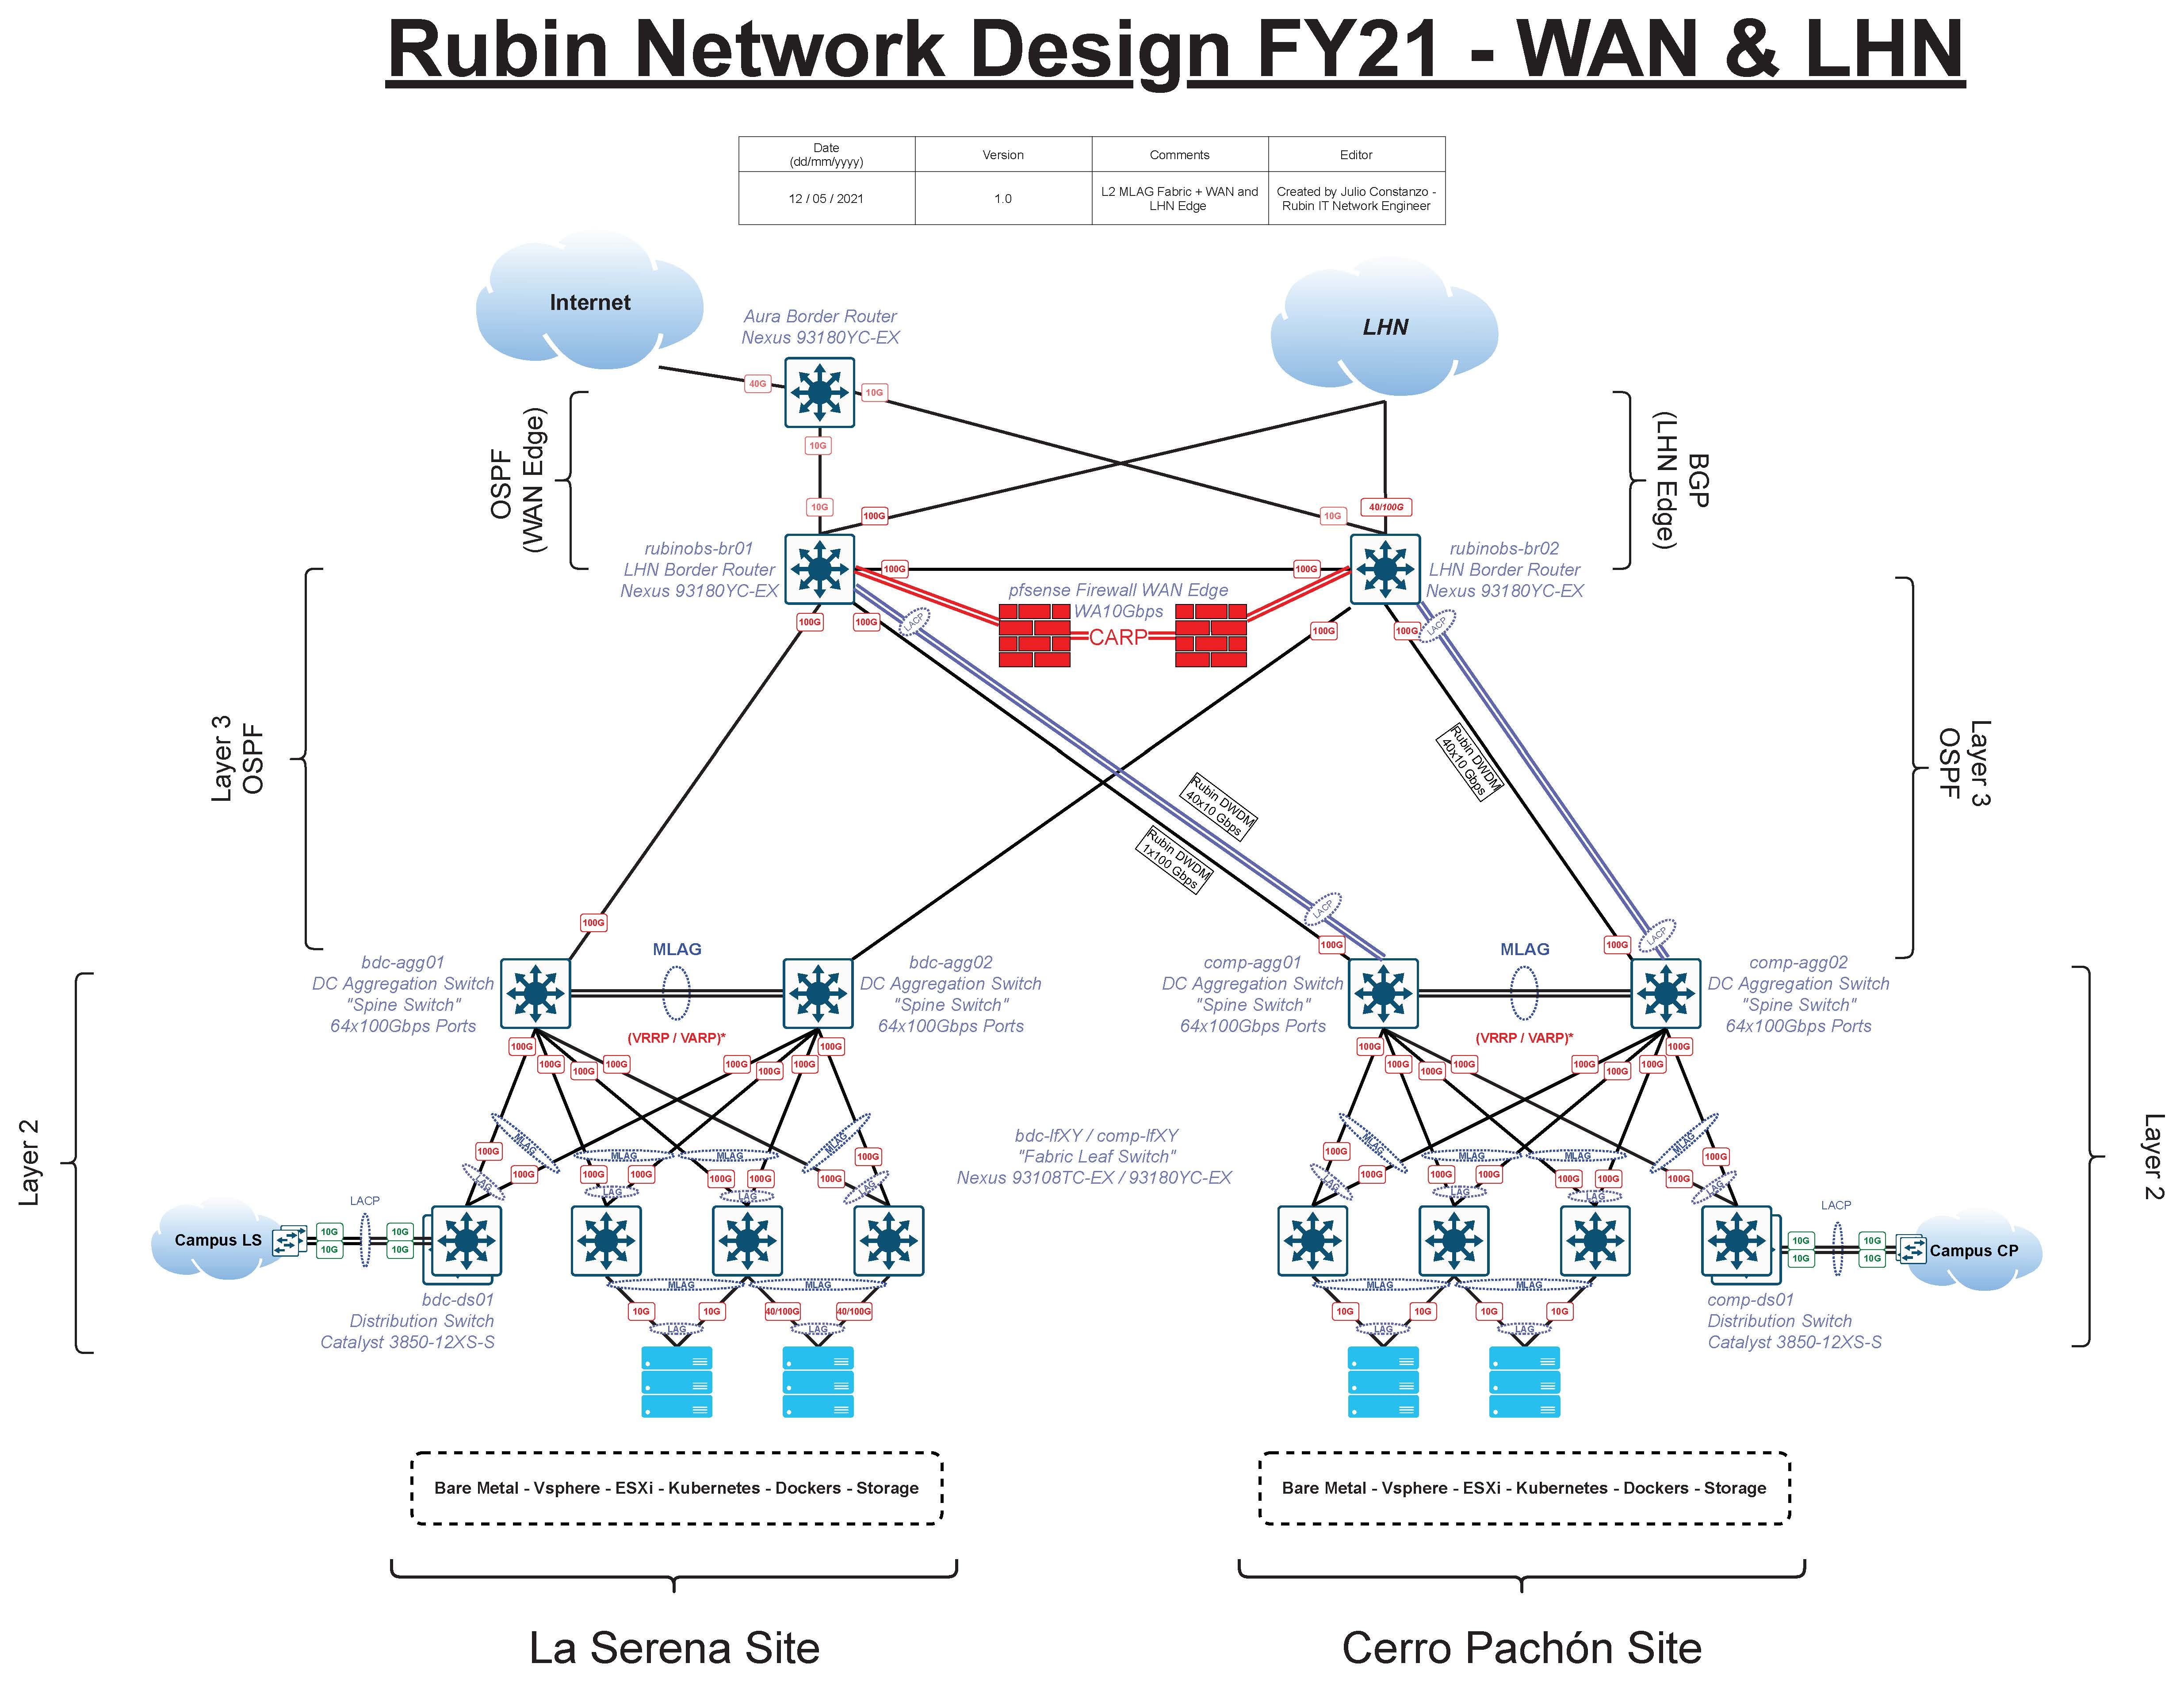
\includegraphics[width=15cm]{images/fy21-rubin-network.jpg}
    \centering
    \caption{FY21 Rubin Network Re-Design}
  \end{figure}

\newpage